% --------------------------------------------------------------------------- %
% Poster about FURAX: A Novel Approach to Optimize Clustering of Parametric  %
% Map-Based Component Separation for Upcoming CMB Polarization Satellites     %
% --------------------------------------------------------------------------- %
% Created using Brian Amberg's LaTeX Poster Template                         %
% Content adapted from the FURAX component separation paper                  %
% --------------------------------------------------------------------------- %

\documentclass[a2paper,portrait,fontscale=0.9]{baposter}

\usepackage{relsize}		% For \smaller
\usepackage{url}			% For \url
\usepackage{graphicx} % Required for resizing symbols
\usepackage{enumitem} % Required for customizing lists
\usepackage{caption}
\usepackage{xcolor} % Required for colors
\usepackage{pifont}
\usepackage{amsmath}
\usepackage{amssymb}
\usepackage{natbib}
\usepackage{svg}
\usepackage{listings}
\usepackage{xcolor} % Make sure xcolor is loaded before listings for color definitions

% Define a custom style for Python code
\lstdefinestyle{custompy}{
    language=Python,
    basicstyle=\footnotesize\ttfamily, % Use a small, monospaced font
    keywordstyle=\color{blue}\bfseries,
    stringstyle=\color{purple},
    commentstyle=\color{gray},
    numbers=none,
    showstringspaces=false,
    breaklines=true, % Automatically break long lines
    frame=none, % No frame around the code
    backgroundcolor=\color{white}, % Set a background color if needed
    tabsize=2
}

\newlist{arrowlist}{itemize}{1}
\setlist[arrowlist]{label=$\resizebox{!}{5pt}{\textbullet}$}
\newcommand{\highlight}[1]{\textbf{\textcolor{red}{#1}}}

\definecolor{darkblue}{rgb}{0.0, 0.0, 0.5}
%%% Global Settings %%%%%%%%%%%%%%%%%%%%%%%%%%%%%%%%%%%%%%%%%%%%%%%%%%%%%%%%%%%

\graphicspath{{figures/}}	% Root directory of the pictures 

%%% Color Definitions %%%%%%%%%%%%%%%%%%%%%%%%%%%%%%%%%%%%%%%%%%%%%%%%%%%%%%%%%

\definecolor{bordercol}{RGB}{40,40,40}
\definecolor{headercol1}{RGB}{186,215,230}
\definecolor{headercol2}{RGB}{80,80,80}
\definecolor{headerfontcol}{RGB}{0,0,0}
\definecolor{boxcolor}{RGB}{240,240,255}
\definecolor{highlightbox}{RGB}{255,240,240}

%%%%%%%%%%%%%%%%%%%%%%%%%%%%%%%%%%%%%%%%%%%%%%%%%%%%%%%%%%%%%%%%%%%%%%%%%%%%%%%%
%%% Utility functions %%%%%%%%%%%%%%%%%%%%%%%%%%%%%%%%%%%%%%%%%%%%%%%%%%%%%%%%%%

%%% Save space in lists. Use this after the opening of the list %%%%%%%%%%%%%%%%
\newcommand{\compresslist}{
	\setlength{\itemsep}{1pt}
	\setlength{\parskip}{0pt}
	\setlength{\parsep}{0pt}
}

%%%%%%%%%%%%%%%%%%%%%%%%%%%%%%%%%%%%%%%%%%%%%%%%%%%%%%%%%%%%%%%%%%%%%%%%%%%%%%%
%%% Document Start %%%%%%%%%%%%%%%%%%%%%%%%%%%%%%%%%%%%%%%%%%%%%%%%%%%%%%%%%%%%
%%%%%%%%%%%%%%%%%%%%%%%%%%%%%%%%%%%%%%%%%%%%%%%%%%%%%%%%%%%%%%%%%%%%%%%%%%%%%%%

\begin{document}

\typeout{Poster rendering started}

%%% Setting Background Image %%%%%%%%%%%%%%%%%%%%%%%%%%%%%%%%%%%%%%%%%%%%%%%%%%
\background{
	\begin{tikzpicture}[remember picture,overlay]%
	\draw (current page.north west)+(-2em,2em) node[anchor=north west]
	{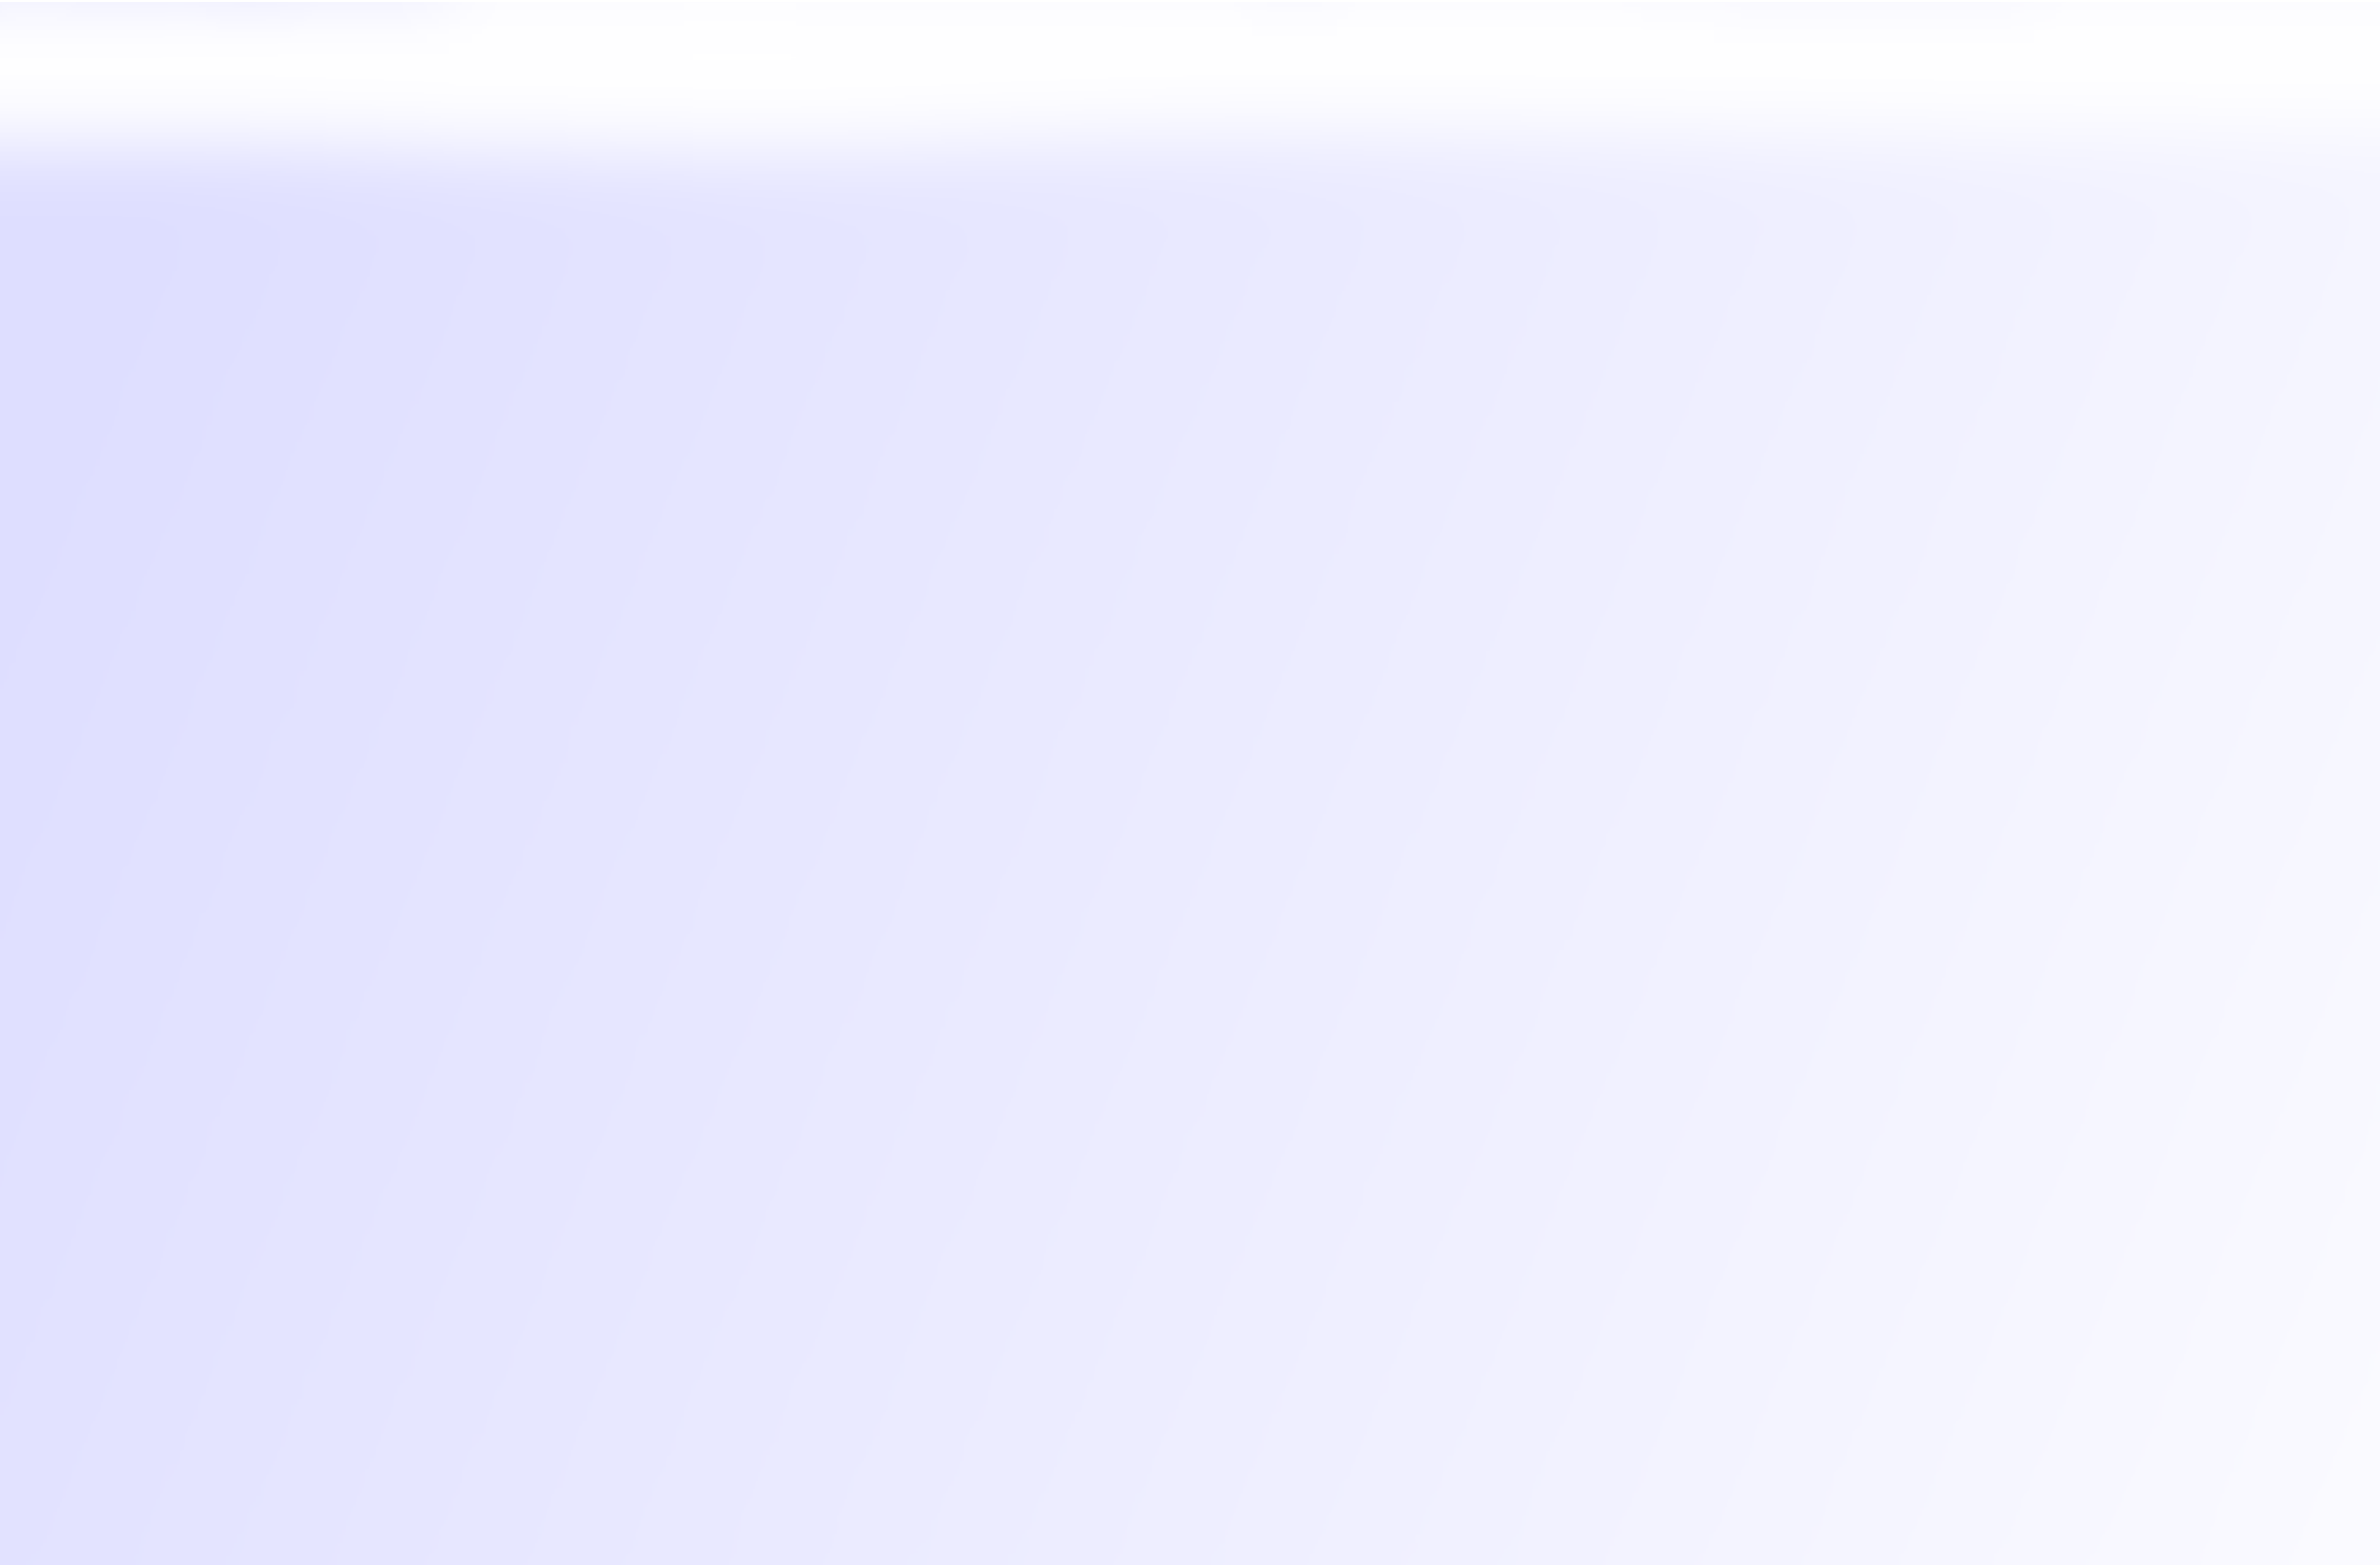
\includegraphics[height=1.1\textheight]{pix/background}};
	\end{tikzpicture}
}

%%% General Poster Settings %%%%%%%%%%%%%%%%%%%%%%%%%%%%%%%%%%%%%%%%%%%%%%%%%%%
%%%%%% Eye Catcher, Title, Authors and University Images %%%%%%%%%%%%%%%%%%%%%%
\begin{poster}{
	grid=false,
	eyecatcher=true, 
	borderColor=bordercol,
	headerColorOne=headercol1,
	headerColorTwo=headercol2,
	headerFontColor=headerfontcol,
	boxColorOne=boxcolor,
	headershape=rounded,
	headerfont=\Large\sf\bf,
	textborder=roundedright,
	background=user,
	headerborder=open,
    columns=2,
    colspacing=2em,
  boxshade=plain
}
%%% Eye Cacther %%%%%%%%%%%%%%%%%%%%%%%%%%%%%%%%%%%%%%%%%%%%%%%%%%%%%%%%%%%%%%%
{
}
%%% Title %%%%%%%%%%%%%%%%%%%%%%%%%%%%%%%%%%%%%%%%%%%%%%%%%%%%%%%%%%%%%%%%%%%%%
{\sf\bf
    A Novel Approach to Optimize Clustering of Parametric Map-Based Component Separation for Upcoming CMB Polarization Satellites
}
%%% Authors %%%%%%%%%%%%%%%%%%%%%%%%%%%%%%%%%%%%%%%%%%%%%%%%%%%%%%%%%%%%%%%%%%%
{
    \vspace{1em} Wassim Kabalan$^{1}$, Wuhyun Sohn$^{1}$, Benjamin Beringue$^{1}$, Artem Basyrov$^{1}$, Pierre Chanial$^{1}$, Alexandre Boucaud$^{1}$, Josquin Errard$^{1}$\\
    \vspace{1em}
    {\footnotesize 
        $^{1}$Université Paris Cité, CNRS, Astroparticule et Cosmologie, F-75013 Paris, France
    }
}
%%% Logo %%%%%%%%%%%%%%%%%%%%%%%%%%%%%%%%%%%%%%%%%%%%%%%%%%%%%%%%%%%%%%%%%%%%%%
{
% The logos are compressed a bit into a simple box to make them smaller on the result
\setlength\fboxsep{0pt}
\setlength\fboxrule{0.5pt}
	\fbox{
	\begin{minipage}{17em}
		
\includegraphics[width=17em,height=12em]{figures/scipol.jpeg}
	\end{minipage}
	}
}

% =============================================================================
% LEFT COLUMN
% =============================================================================

\headerbox{\textbf{Tensor-to-Scalar Ratio \& Foreground Removal}}{name=motivation,column=0,row=0,boxColorOne=highlightbox}{
\vspace{0.1cm}

\begin{minipage}{0.45\textwidth}
\centering
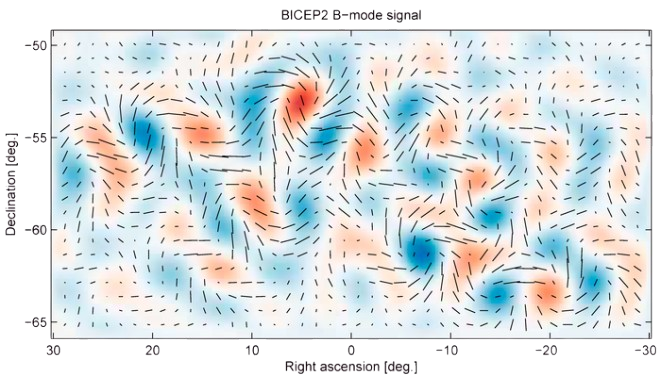
\includegraphics[width=\textwidth]{B-modes.png}
\captionof{figure}{CMB B-mode polarization signal from primordial gravitational waves}
\end{minipage}
\hfill
\begin{minipage}{0.45\textwidth}
\centering
\includesvg[width=\textwidth]{figures/foregrounds.svg}
\captionof{figure}{Galactic foreground contamination}
\end{minipage}

\vspace{0.1cm}

\textbf{The Challenge:}
\begin{itemize}[leftmargin=0.5cm] \compresslist
    \item[\ding{227}] Measuring tensor-to-scalar ratio $r$ requires detecting faint B-mode polarization
    \item[\ding{227}] Galactic foregrounds dominate CMB signal by orders of magnitude
    \item[\ding{227}] \highlight{Accurate foreground removal is critical for $r < 0.001$ detection}
\end{itemize}

\vspace{0.1cm}
}
\headerbox{\textbf{Parametric Component Separation}}{name=parametric,column=0,below=motivation}{
\vspace{0.1cm}

% Begin two-column layout
\textbf{Data Model:}
\begin{equation}
    \mathbf{d} = \mathbf{A}(\boldsymbol{\beta})\,\mathbf{s} + \mathbf{n}
\end{equation}
where $\mathbf{d}$ is observed data, $\mathbf{s}$ are sky components, $\mathbf{A}(\boldsymbol{\beta})$ encodes spectral dependencies, and $\mathbf{n}$ is noise.

\textbf{Generalized Least Squares Solution:}
\begin{equation}
    \hat{\mathbf{s}} = \left( \mathbf{A}^\top \mathbf{N}^{-1} \mathbf{A} \right)^{-1} \mathbf{A}^\top \mathbf{N}^{-1} \mathbf{d}
\end{equation}

\textbf{Spectral Likelihood:}
\begin{equation}
    \ln \mathcal{L}_{\mathrm{spec}}(\boldsymbol{\beta}) \propto (\mathbf{A}^\top \mathbf{N}^{-1} \mathbf{d})^\top (\mathbf{A}^\top \mathbf{N}^{-1} \mathbf{A})^{-1} (\mathbf{A}^\top \mathbf{N}^{-1} \mathbf{d})
\end{equation}

\textbf{Key Innovation:} Data-driven optimization of spatial clustering rather than fixed patching schemes.
\centering % Center all content within this column

\vspace{0.5cm} % Creates a clean separation between the snippet and the plot
% --- FURAX Code Snippet ---
\textbf{FURAX Implementation:}
\fbox{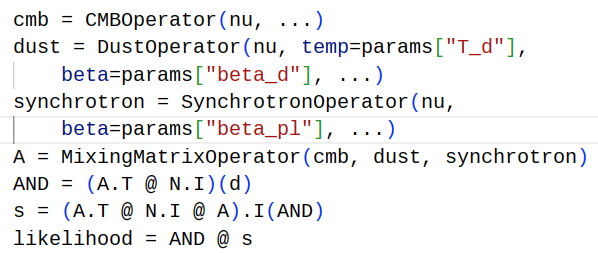
\includegraphics[width=0.8\linewidth]{figures/snippet.png}}
\vspace{0.5cm} % Creates a clean separation between the snippet and the plot

}

\headerbox{\textbf{Spatial Variability}}{name=spatial,column=0,below=parametric}{
\vspace{0.1cm}

\textbf{Foreground Spectral Parameters Vary Across Sky:}

\begin{center}
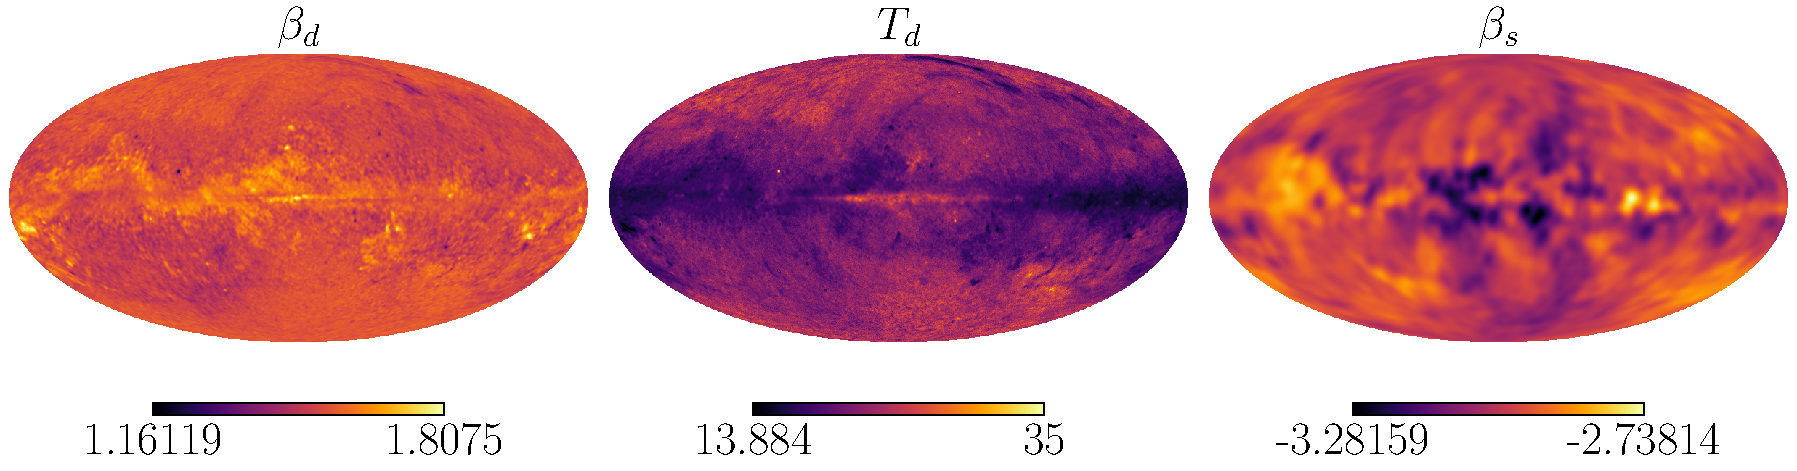
\includegraphics[width=0.8\textwidth]{mbb_index_map.pdf}
\captionof{figure}{Modified blackbody spectral index map showing spatial variability in dust emission properties across the sky}
\end{center}

\textbf{Clustering Approach:}
\begin{itemize}[leftmargin=0.5cm] \compresslist
    \item[\ding{227}] Spherical K-means clustering groups pixels with similar spectral properties
    \item[\ding{227}] Balances statistical uncertainty with modeling flexibility
\end{itemize}

\vspace{0.1cm}

\textbf{Optimized K-means Parameters:}
\begin{center}
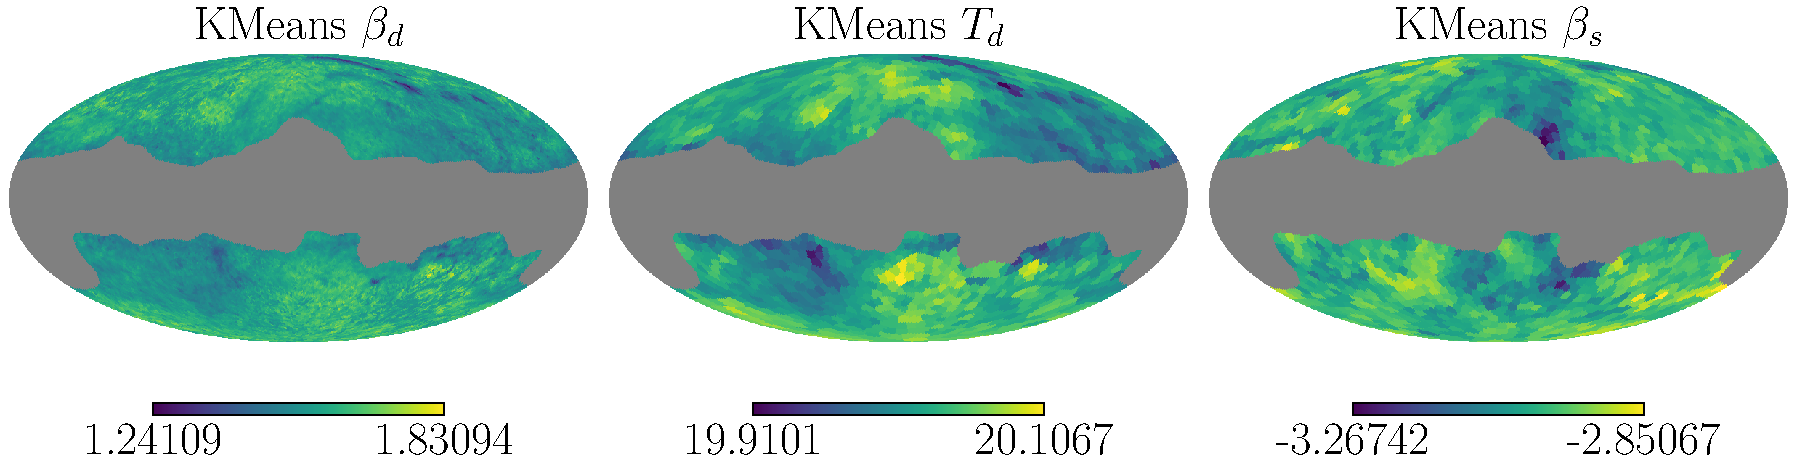
\includegraphics[width=0.7\textwidth]{params_KMeans.pdf}
\captionof{figure}{Optimized spectral parameter distributions from K-means clustering showing data-driven adaptation to foreground complexity}
\end{center}

\vspace{0.1cm}
}


% =============================================================================
% RIGHT COLUMN
% =============================================================================


\headerbox{\textbf{The FURAX Framework}}{name=furax,column=1,row=0,span=1}{

\vspace{0.1cm}

\begin{minipage}{0.45\textwidth}
    
    \begin{itemize}[leftmargin=0.5cm] \compresslist

        \item[\ding{227}] \textbf{JAX-Native}: Differentiable \& GPU accelerated
        \item[\ding{227}] \textbf{Modular Design}: Composable algebraic operators
        \item[\ding{227}] \textbf{Memory Efficient}: Matrix-free linear operators
        \item[\ding{227}] \textbf{Scalable}: Multi-GPU execution

    \end{itemize}


    \textbf{Grid Search}: Configuration space $\mathcal{G} = \{K_{\beta_d}\} \times \{K_{T_d}\} \times \{K_{\beta_s}\}$ evaluated across 1.92M component separation runs.

    \vspace{0.3cm} % Creates a clean separation between the snippet and the plot
    % --- Runtime Comparison Plot ---
    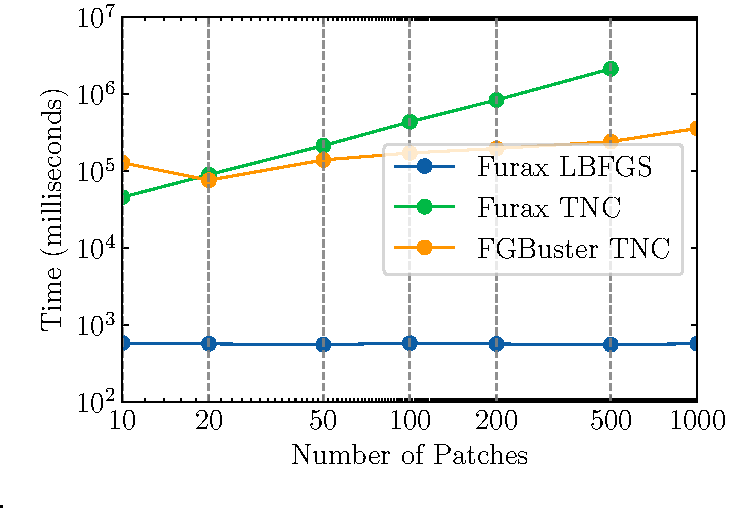
\includegraphics[width=\linewidth]{figures/runtime_comparison.pdf}
    \captionof{figure}{Runtime comparison of FURAX Component Separation}

\end{minipage}
\hfill
\begin{minipage}{0.45\textwidth}
    \begin{center}
        \includesvg[width=0.9\textwidth]{figures/FURAX-CS.svg}
        
        \captionof{figure}{FURAX pipeline: Grid search over clustering configurations, spectral parameter optimization, and CMB variance minimization for model selection}
    \end{center}
    \end{minipage}    


\vspace{0.2cm}

} 



\headerbox{\textbf{Likelihood and Variance Analysis}}{name=analysis,column=1,below=furax}{
\vspace{0.3cm}

\textbf{Selection Criterion - CMB Variance Minimization:}
\begin{equation}
    \sigma^2_{\mathrm{CMB}} = \left\langle \mathrm{Var}_{i} \left[ \hat{s}^{(i)}_{\mathrm{CMB}} \right] \right\rangle_{\text{pixels}}
\end{equation}

\begin{center}
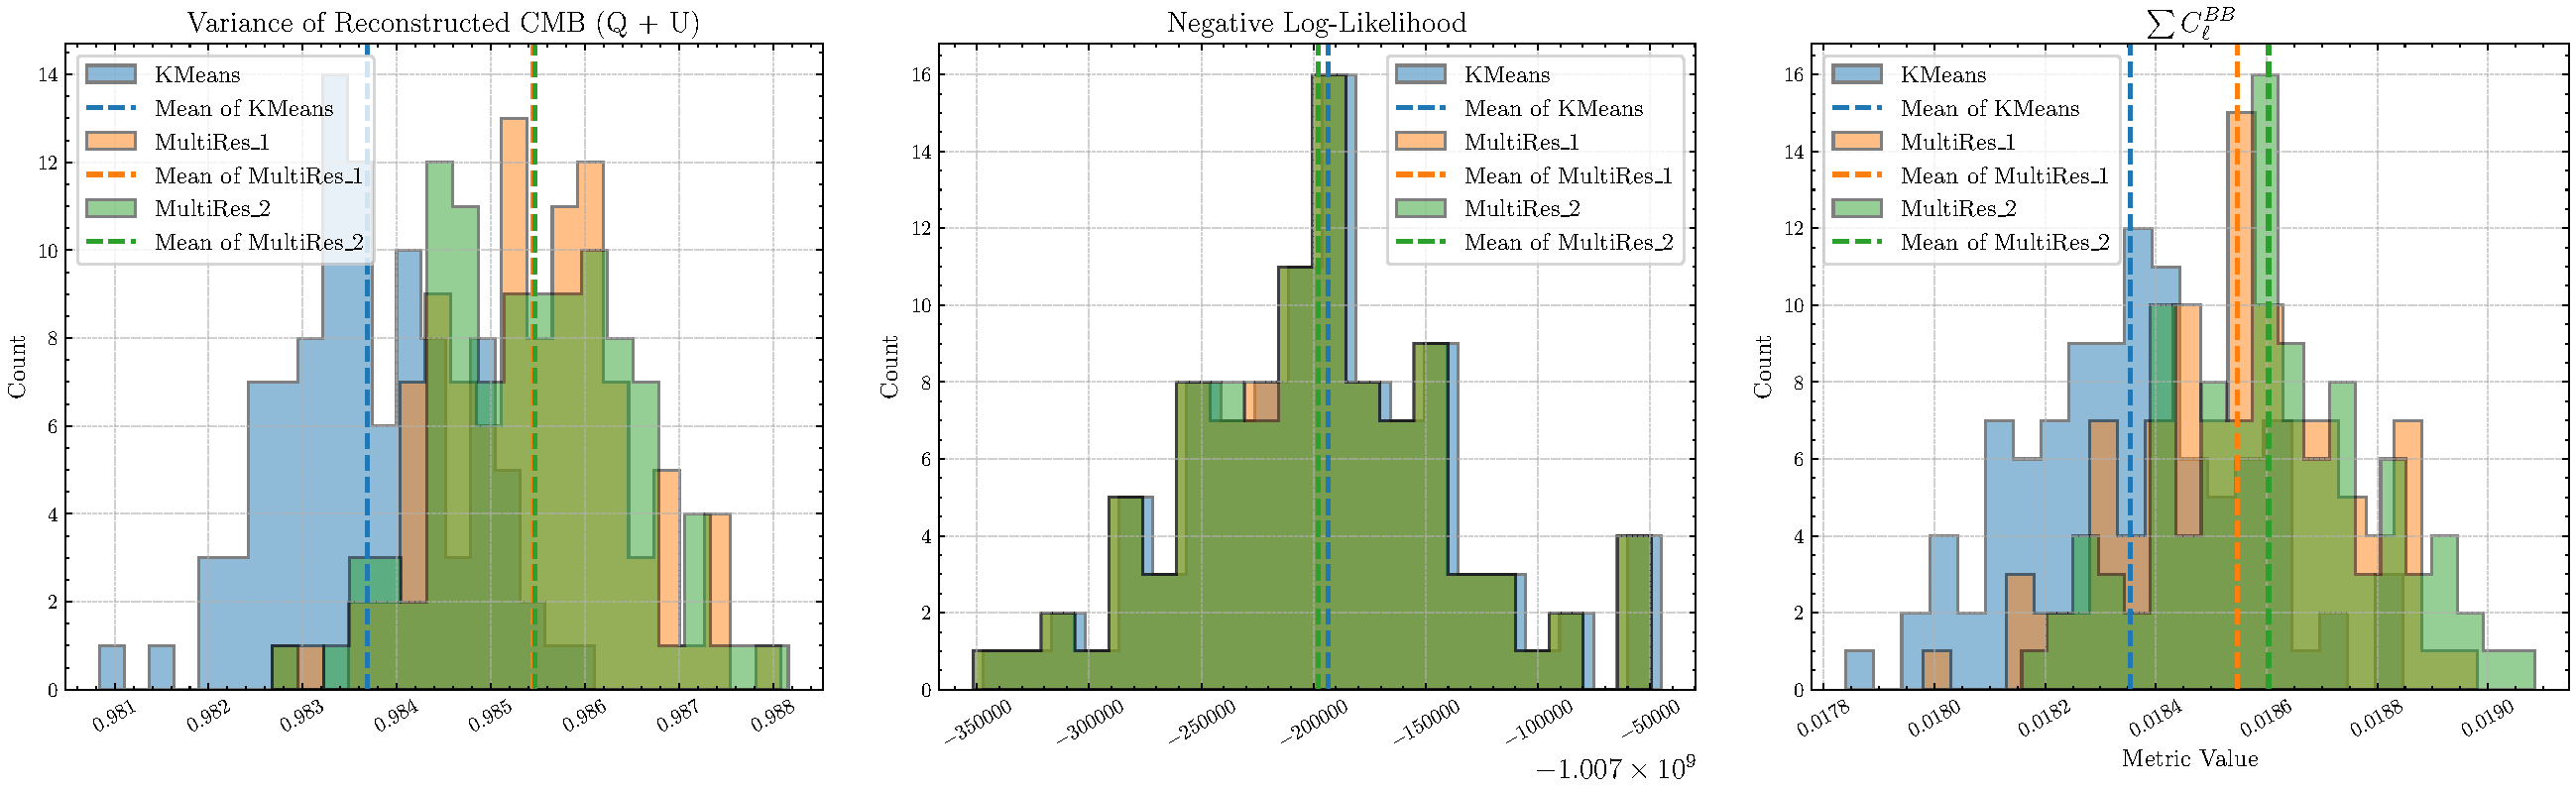
\includegraphics[width=1.0\textwidth]{variance_likelihood_distributions.pdf}
\captionof{figure}{Distribution of CMB variance, spectral likelihood, and B-mode power for different spatial modeling approaches. K-means clustering achieves optimal balance.}
\end{center}

\textbf{Key Insight:} Variance minimization acts as proxy for residual foreground contamination, leading to more robust cosmological constraints.

\vspace{0.2cm}
}

\headerbox{\textbf{Results}}{name=results,column=1,below=analysis,span=1}{
\vspace{0.3cm}

\begin{minipage}{0.48\textwidth}

    \textbf{Tensor-to-Scalar Ratio Constraints:}

    \begin{center}
    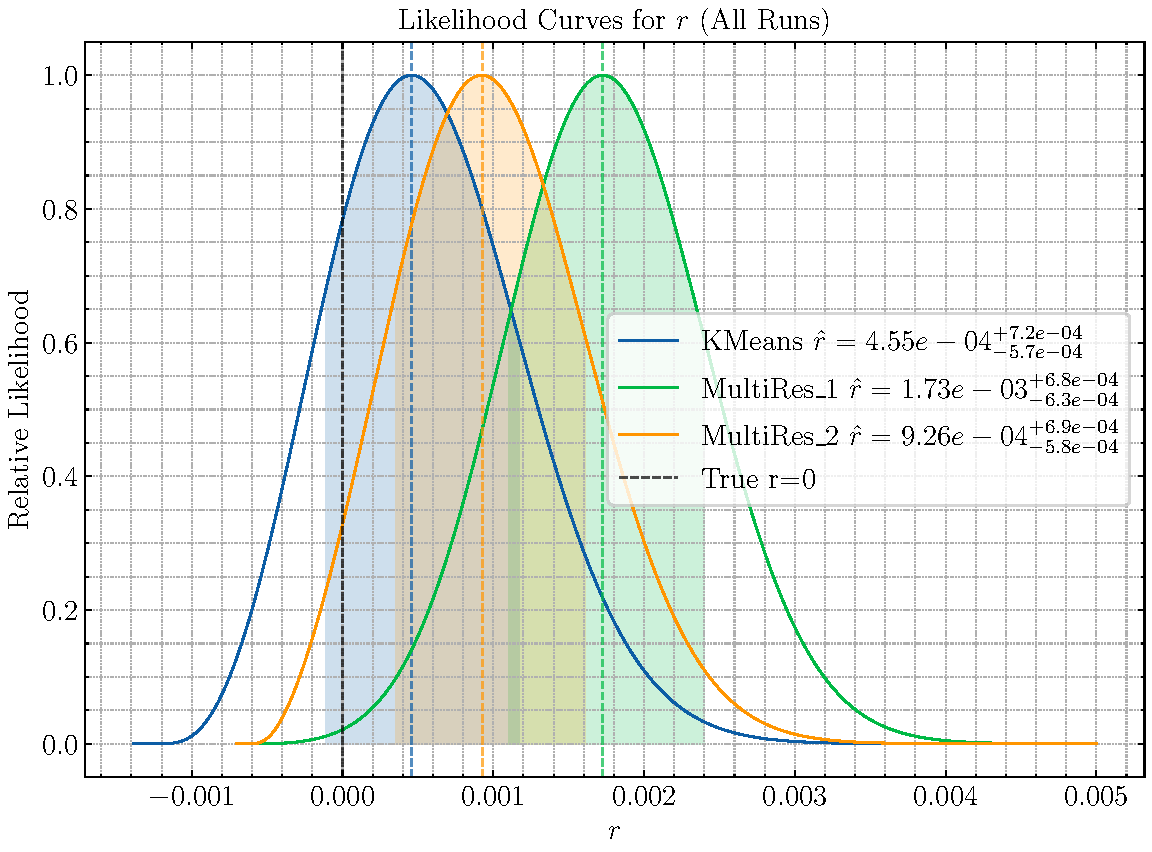
\includegraphics[width=1.0\textwidth]{r_likelihood_distribution.pdf}
    \captionof{figure}{$r$ likelihood distributions: K-means clustering (blue) yields $\hat{r} = 4.55 \times 10^{-4}$ with lowest bias and tightest constraints compared to multi-resolution approaches}
    \end{center}

\end{minipage}
\hfill
\begin{minipage}{0.48\textwidth}

    \textbf{Residual B-mode Spectra:}
    \begin{center}
    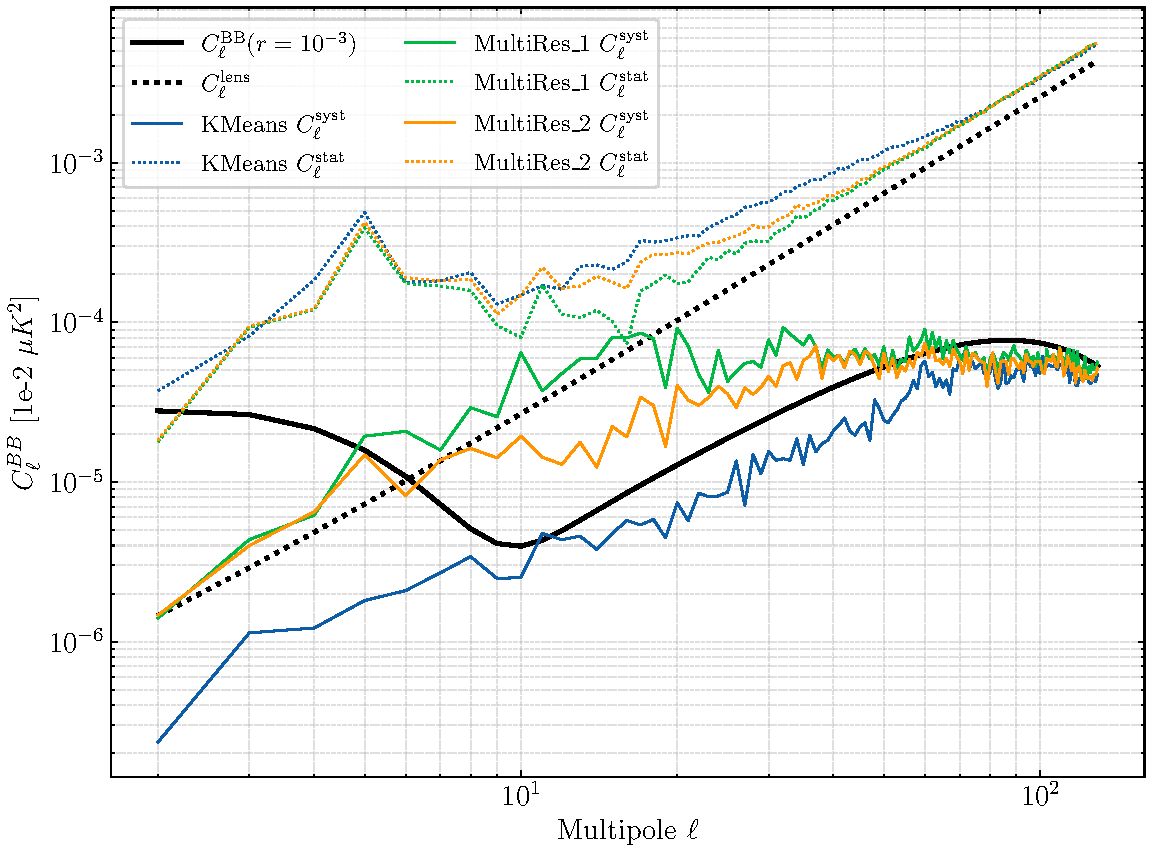
\includegraphics[width=1.0\textwidth]{bb_residual_spectra.pdf}
    \captionof{figure}{Residual B-mode power spectra: K-means clustering (blue) achieves significantly lower systematic residuals compared to multi-resolution approaches, falling below target sensitivity levels}
    \end{center}
\end{minipage}

\vspace{0.2cm}
}

% =============================================================================
% BOTTOM SECTION - REFERENCES
% =============================================================================

\headerbox{\textbf{References \& Acknowledgements}}{name=references,column=0,below=results,span=2,below=spatial}{
\vspace{0.4em}

\textbf{Key References:}
\begin{itemize}[leftmargin=0.5cm] \compresslist
    \item FURAX framework \& component separation methodology: Kabalan et al. (2024), arXiv:2024.xxxxx
    \item LiteBIRD collaboration forecasts: LiteBIRD Collaboration (2022), PTEP 2023
    \item JAX ecosystem for scientific computing: Bradbury et al. (2018), JAX library
\end{itemize}

\textbf{Acknowledgements:} This work was supported by the \textsc{SciPol} project (ERC Grant No. 101044073, PI: Josquin Errard) and performed using HPC resources at IDRIS Jean Zay supercomputer. Full code available at: \url{https://github.com/ASKabalan/furax-compsep-paper}

\vspace{0.2cm}
}

\end{poster}
\end{document}